\documentclass{article}
\usepackage{graphicx}
\usepackage{amsmath}
\usepackage{amsthm}
\usepackage{amsfonts}
\usepackage{mathtools}
\usepackage{xfrac}
\usepackage{float}
\usepackage[T1]{fontenc}
\usepackage[utf8]{inputenc}

\graphicspath{ {./pictures/} }
\DeclareGraphicsExtensions{.pdf, .png}

\newtheorem{theorem}{Theorem}
\newtheorem{lemma}{Lemma}
\newtheorem{proposition}{Proposition}
\newtheorem{corollary}{Corollary}

\newcommand{\apply}[2]{\left\langle#1, #2\right\rangle}
\newcommand{\prob}[1]{\mathrm{P}{\left[#1\right]}}
\newcommand{\Var}{\mathrm{Var}}
\newcommand{\E}{\mathrm{E}}
\newcommand{\J}{J^{(\alpha)}}
\usepackage{todonotes}

\makeatletter
\newcommand{\subalign}[1]{%
  \vcenter{%
    \Let@ \restore@math@cr \default@tag
    \baselineskip\fontdimen10 \scriptfont\tw@
    \advance\baselineskip\fontdimen12 \scriptfont\tw@
    \lineskip\thr@@\fontdimen8 \scriptfont\thr@@
    \lineskiplimit\lineskip
    \ialign{\hfil$\m@th\scriptstyle##$&$\m@th\scriptstyle{}##$\hfil\crcr
      #1\crcr
    }%
  }%
}
\makeatother


\begin{document}

\section{Introduction}

\todo[inline]{MD: I am going to write some quick comments/remarks
  using this environment}

\todo[inline]{MD: It would be good to add a context: quick comments on
random matrices GUE/GOE/GSE and G$\beta$E as their generalization
(what's their definition? who
was studyingn them before? which important results were obtained
before that motivate your research?);
classical law of large numbers starting from Wigner and going to
Johansson with the universal semicircle law limit. Then the most
recent results about the ``high-temperature'' limit (it would be good
to mention that the ``high temperature'' comes from the log-gas system
interpretation where $\beta$ is the inverse of the temperature of the
model. Impartant: the purpose of the introduction is to give a context
and motivation for your study; at the same time it should be
mathematically as light as possible.}

Recall, that 'eigenvalues' distrubution of Gaussian $\beta$-ensemble of size $N$ has density
$$
    	\frac{1}{Z_{N}^{(\beta)}}\exp{\left(-\frac{1}{2}\sum\limits_{i = 1}^{N}x_{i}^2\right)}|V_N(x_1, \ldots, x_N)|^{\beta},
		$$
		where $V_N$ is a Vandermonde determinant:
        $$
            V_N(x_1, \ldots, x_{N}) = \prod\limits_{i = 1}^{N}\prod\limits_{j = i + 1}^{N}|x_i - x_j| 
        $$
        and $Z_{N}^{(\beta)}$ is just a normalization coefficient:
		$$
			Z_{N}^{(\beta)} = 
        \int\limits_{\mathbb{R}^N}\exp{\left(-\frac{1}{2}\sum\limits_{i = 1}^{N}x_{i}^2\right)}|V_N(x_1, \ldots, x_N)|^{\beta}.
		$$
    We denote this density by $g_N^{(\beta)}(x_1, \ldots, x_N)$.

    The goal of this paper is, in certain sense, describe the asymptotic behaviour of a random vector
    $$
        (\lambda_{1}^{(\beta)}, \ldots, \lambda_{N}^{(\beta)}) \propto g_{N}^{(\beta)},
    $$
    when $N \to +\infty$ while $N \cdot \beta \to 2c$, where $c$ is
    some constant.

    \todo[inline]{MD: Did someone study this problem before? Why your
      result is better (hint: elementary proof as in the case of the
      finite $\beta$; proof that does not require the tridiagonal
      model -> potential to generalize to other measures; new
      connection between high-temperature limit and maps on
      surfaces;)}

    To be more precise, we introduce the random measure
    $$
        L_{N}^{(\beta)} = \frac{1}{N}\sum\limits_{i = 1}^{N}\delta_{\sfrac{\lambda_{N}^{(\beta)}}{\sqrt{N}}},
    $$
    where $\delta_{a}$ is a Dirac measure.

    
    Then fix any sequence of positive integers $\{N_m\}_{m = 1}^{\infty}$ and positive reals $\{\beta_{m}\}_{m = 1}^{\infty}$ such that
    $$
        \lim\limits_{m \to \infty}N_m = +\infty \text{ and } \lim\limits_{m \to \infty}N_m\beta_m = 2c,
    $$
    for some constant $c$ and set $L_m \coloneqq L_{N_m}^{(\beta_m)}$. Denote by $\overline{L}_m$ the mean of $L_m$: $\forall f \in C_{b}(\mathbb{R}), \, \apply{\overline{L}_m}{f} = \E\left[\apply{L_m}{f}\right]$.
    
    We prove that moments of $\overline{L}_m$ converge to the following sequence:

$$
    \begin{cases}
        M_{2k + 1} = 0 & k \geq 0 \\
		M_{2k} = \sum\limits_{r + s = k - 1}M_{2r}M_{2s} + c(2k - 1)M_{2k - 2} & k > 0 \\
		M_{2k} = 1 & k = 0.
	\end{cases}
$$

    \begin{proposition}\label{prop:moments}
    For every non-negative integer $k$:
    $$
    \lim\limits_{m \to \infty}\apply{\overline{L}_m}{x^k} = M_{k}
    $$
    \end{proposition}

    We also prove, that the variance of moments of $L_m$ tends to $0$:
    
    \begin{proposition}\label{prop:variance}
    For every positive integer $k$:
    $$
    \lim\limits_{m \to \infty}\Var\left[\apply{L_m}{x^k}\right] = 0
    $$
    \end{proposition}

    These two propositions together imply the main result of this paper:
    
    \begin{theorem}\label{theorem:main}
        There is a unique measure $L$, whose $k$-th moments are $M_k$ and $L_m$ converges weakly, in probability to $L$. Precisely:
        
        For all $\epsilon > 0$ and $f \in C_b(\mathbb{R})$:
        $$
            \lim\limits_{m \to \infty}\prob{\left|\apply{L_m}{f} - \apply{L}{f}\right| > \epsilon} = 0
        $$
    \end{theorem}

    \todo[inline]{MD: Again, it is good to think what is the main
      result. The main result is the LLN for your model. The novelty
      is the method - it's purely combinatorial. It is not necessary
      to state propositions separately in the introduction; it's
      better to ezplain in words that you will prove purely
      combinatoriall the convergence of moments, and you will deduce
      the main theorem using a standard arguement that shows that
      variance is small.}

    \section{Connections to $h$-coefficients}

        \todo[inline]{MD: Jack polynomials should be introduced. It is
        not necessary to define them from scratch, but some references
      should be used (warning you mixed x's with y's).}

    First we state the main result of \cite{Okounkov_1997}, which connects $\beta$-distribition to Jack polynomials.

    Denote by $\left[|y|^{|\lambda|}\right]\J_{\lambda}(y)$ the coefficient of the polynomial $(\sum{x_i^2})^{\sfrac{|\lambda|}{2}}$ in the power-sum expansion of $\J_{\lambda}(y)$.

    Then the following holds true:

    \begin{equation}\label{eq:okounkov}
        \int\limits_{\mathbb{R}^n}\J_\lambda(t)g_{N}^{(\sfrac{2}{\alpha})}(t)\mathop{dt} = \J_{\lambda}(1, \ldots, 1)\left(\left[ |y|^{|\lambda|}\right]\J_\lambda(y)\right).
      \end{equation}

              \todo[inline]{MD: It's hard to find what's $g_N$. It
                would be better to introduced it by equation, to which
                you can refer.}

    We rewrite it as follows:
    \begin{equation}\label{eq:okounkov}
        \int\limits_{\mathbb{R}^n}\J_\lambda(t)g_{N}^{(\sfrac{2}{\alpha})}(t)\mathop{dt} = \J_{\lambda}(x)\J_{\lambda}(y)\Bigg|_{\subalign{
            &p_r(x) = N \\
            &p_r(y) = \delta_{r, 2}
        }},
    \end{equation}

    meaning, that we expand $\J_{\lambda}(x)$ and $\J_{\lambda}(y)$ in the power-sum basis and for every integer $r \geq 0$ we substitute $N$ instead of $p_r(x)$ and $\delta_{r, 2}$ instead of $p_r(y)$, where $\delta$ is a Kronecker delta.

\begin{lemma}\label{lemma:moments_and_jack}
    For any partition $\theta \vdash m$:
    \begin{equation}        
    \int\limits_{\mathbb{R}^N}p_{\theta}(t)g_N^{(\sfrac{2}{\alpha})}(t)\mathop{dt} = z_{\theta}\alpha^{l(\theta)}[p_{\theta}(z)]\left.\left(
    \sum\limits_{\lambda}
    \frac{\J_{\lambda}(x)\J_{\lambda}(y)\J_{\lambda}(z)}{\langle \J_{\lambda} \J_{\lambda}\rangle_{\alpha}}\right)\right |_{\subalign{
            &p_r(x) = N \\
            &p_r(y) = \delta_{r, 2}
        }}
    \end{equation}
         \todo{MD: $z_\theta$ not defined}
\end{lemma}
\begin{proof}
    Note, that:
    \begin{equation}\label{eq:lemma1:first}
        \frac{1}{z_{\theta}\alpha^{l(\theta)}}\int\limits_{\mathbb{R}^N}p_{\theta}(t)g_N^{(\sfrac{2}{\alpha})}(t)\mathop{dt} = [p_{\theta}(z)]\int\limits_{\mathbb{R}^N}\left(\sum\limits_{\lambda \vdash m}\frac{p_{\lambda}(z)p_{\lambda}(t)}{z_{\lambda}\alpha^{l(\lambda)}}\right)g_N^{(\sfrac{2}{\alpha})}(t)\mathop{dt}.
    \end{equation}

    Now we use the Cauchy identity \todo{MD: add the preliminary
      section (where Jack polynomials are defined) with important
      results such as the Cauchy identity}:
    $$
		\prod_{i, j}(1 - x_iy_j)^{-\frac{1}{\alpha}} = \sum_{\lambda}{\frac{p_{\lambda}(x)p_{\lambda}(y)}{z_{\lambda}\alpha^{l(\lambda)}}} = \sum_{\lambda}{\frac{\J_{\lambda}(x)\J_{\lambda}(y)}{\langle \J_{\lambda}, \J_{\lambda}\rangle_{\alpha}}},
	$$
    to switch from power sum symmetric functions to Jack polynomials and apply (\ref{eq:okounkov}):

    \begin{multline}\label{eq:lemma1:second}
        \int\limits_{\mathbb{R}^N}\left(\sum\limits_{\lambda \vdash m}\frac{p_{\lambda}(t)p_{\lambda}(z)}{z_{\lambda}\alpha^{l(\lambda)}}\right)g_N^{(\sfrac{2}{\alpha})}(t)\mathop{dt} =
		\int\limits_{\mathbb{R}^N}\left(\sum\limits_{\lambda \vdash m}\frac{\J_{\lambda}(t)\J_{\lambda}(z)}{\langle \J_{\lambda}, \J_{\lambda}\rangle_{\alpha}}\right)g_N^{(\sfrac{2}{\alpha})}(t)\mathop{dt} = \\
        \sum\limits_{\lambda \vdash m}\frac{\J_{\lambda}(z)}{\langle \J_{\lambda}, \J_{\lambda}\rangle_{\alpha}}\int\limits_{\mathbb{R}^N}\J_{\lambda}(t)g_N^{(\sfrac{2}{\alpha})}(t)\mathop{dt} = \\
    	\left.\sum\limits_{\lambda \vdash m}
		\frac{\J_{\lambda}(x)\J_{\lambda}(y)\J_{\lambda}(z)}
		{\langle \J_{\lambda}, \J_{\lambda}\rangle_{\alpha}}
		\right\vert_{\subalign{&p_r(x) = N \\ &p_r(y) = \delta_{r, 2}}}
    \end{multline}
    Combining (\ref{eq:lemma1:first}) and (\ref{eq:lemma1:second}) gives the desired result.
\end{proof}

    Denote
    $$
	   \phi(x, y, z; t, \alpha) = \sum\limits_{n \geq 0 }t^n\sum\limits_{\lambda \vdash n}\frac{\J_{\lambda}(x)\J_{\lambda}(y)\J_{\lambda}(z)}{\langle \J_{\lambda}, \J_{\lambda}\rangle_{\alpha}}
    $$
    and
    \begin{equation}\label{eq:psi}  
	   \psi(x, y, z; t, \alpha) = \alpha t\frac{\partial}{\partial t}\log{(\phi)} =
	   \sum\limits_{n\geq 1}t^n
	   \left(\sum\limits_{\mu, \nu, \tau \vdash n}h_{\mu, \nu}^{\tau}(\alpha - 1)p_{\mu}(x)p_{\nu}(y)p_{\tau}(z)\right).
    \end{equation}

Now we are ready to prove the crucial lemma:
\begin{lemma}\label{lemma:moments_and_h}
    For any partition $\theta \vdash m$:
    \begin{multline}
        \int\limits_{\mathbb{R}^N}p_{\theta}(t)g_N^{(\sfrac{2}{\alpha})}(t)\mathop{dt} = \\ z_{\theta}\alpha^{l(\theta)}[t^mp_{\theta}(z)]\exp\left(\frac{1}{\alpha}\sum\limits_{n \geq 1}\frac{t^{2n}}{2n}\sum\limits_{\mu, \tau \vdash 2n}h_{\mu, (2)^n}^{\tau}(\alpha - 1)N^{l(\mu)}p_{\tau}(z)\right).
      \end{multline}
    In particular
    $$
        \int\limits_{\mathbb{R}^N}p_{\theta}(t)g_N^{(\sfrac{2}{\alpha})}(t)\mathop{dt} = 0,
    $$
    unless $m$ is even.
\end{lemma}
\begin{proof}
    First, we note that:
    \begin{multline}\label{eq:lemma2:1}
        [p_{\theta}(z)]\left.\left(
    \sum\limits_{\lambda}
    \frac{\J_{\lambda}(x)\J_{\lambda}(y)\J_{\lambda}(z)}{\langle \J_{\lambda} \J_{\lambda}\rangle_{\alpha}}\right)\right |_{\subalign{
            &p_r(x) = N \\
            &p_r(y) = \delta_{r, 2}
        }} = \\ = [t^mp_{\theta}(z)]\phi(x, y, z; t, \alpha)\Big|_{
        \subalign{
            &p_r(x) = N \\
            &p_r(y) = \delta_{r, 2}
        }
        }
    \end{multline}
    From (\ref{eq:psi}) we deduce:
    \begin{multline}\label{eq:lemma2:2}
        \phi(x, y, z; \alpha) = \exp{\left(\int\frac{\psi(x, y, z; \alpha)}{\alpha t}\mathop{dt}\right)} = \\ \exp\left(\frac{1}{\alpha}\sum\limits_{n \geq 1}\frac{t^n}{n}
	   \left(\sum\limits_{\mu, \nu, \tau \vdash n}h_{\mu, \nu}^{\tau}(\alpha - 1)p_{\mu}(x)p_{\nu}(y)p_{\tau}(z)\right) \right)
       \end{multline}
       \todo{MD: This integral might make no sense - it would be better
       to say that you want to take the formal antiderivative}
    Note, that:
    $$
    p_{\mu}(x)\big|_{p_r(x) = N} = N^{l(\mu)} \text{ and } p_{\nu}(y)\big|_{p_r(y) = \delta_{r, 2}} =
    \begin{cases}
         1 & \nu = (2^{\sfrac{l(\nu)}{2}}) \\
         0 & \text{ otherwise }
    \end{cases}.
    $$
    In particular, $p_{\nu}(y)\big|_{p_r(y) = \delta_{r, 2}} = 0$ unless the size of $\nu$ is even. Now we are ready to do the corresponding substitutions in (\ref{eq:lemma2:2}) to obtain:
    \begin{equation}\label{eq:lemma2:3}
        \phi(x, y, z; t, \alpha)\Big|_{
        \subalign{
            &p_r(x) = N \\
            &p_r(y) = \delta_{r, 2}
        }
        } = \exp\left(\frac{1}{\alpha}\sum\limits_{n \geq 1}\frac{t^{2n}}{2n}\sum\limits_{\mu, \tau \vdash 2n}h_{\mu, (2)^n}^{\tau}(\alpha - 1)N^{l(\mu)}p_{\tau}(z)\right).
    \end{equation}
    The rest is just combining (\ref{eq:lemma2:1}),  (\ref{eq:lemma2:3}) and \textbf{Lemma \ref{lemma:moments_and_jack}}.
\end{proof}

\begin{proposition}\label{prop:moments_and_h}
    For all positive integers $k$ the following holds:
    \begin{equation}
        \begin{cases}
        \langle \overline{L}_{N}^{(\sfrac{2}{\alpha})}, x^{2k + 1} \rangle = 0 \\
        \langle \overline{L}_{N}^{(\sfrac{2}{\alpha})}, x^{2k} \rangle = \frac{1}{N^{k + 1}}\sum\limits_{\mu \vdash 2k}h_{\mu, (2^k)}^{(2k)}(\alpha - 1)N^{l(\mu)}
        \end{cases}
    \end{equation}
\end{proposition}
\begin{proof}
    Note, that:
    $$
        \langle \overline{L}_{N}^{(\sfrac{2}{\alpha})}, x^{r} \rangle = \E\left[\frac{1}{N}\sum\limits_{i = 1}^N\left(\frac{\lambda_i}{\sqrt{N}}\right)^r\right] = \frac{1}{N^{1 + \sfrac{r}{2}}}\int\limits_{\mathbb{R}^N}p_{(r)}(t)g_N^{(\sfrac{2}{\alpha})}\mathop{dt}.
        $$
        \todo{$\E$ is not defined}
    It follows from \textbf{Lemma \ref{lemma:moments_and_h}}, that:
    $$
        \langle \overline{L}_{N}^{(\sfrac{2}{\alpha})}, x^{2k + 1} \rangle = 0
    $$
    Now for brevity, denote:
    $$
        A(t) = \frac{1}{\alpha}\sum\limits_{n \geq 1}\frac{t^{2n}}{2n}\sum\limits_{\mu, \tau \vdash 2n}h_{\mu, (2)^n}^{\tau}(\alpha - 1)N^{l(\mu)}p_{\tau}(z).
    $$
    \textbf{Lemma \ref{lemma:moments_and_h}} says, that:
    $$
        \int\limits_{\mathbb{R}^N}p_{(r)}(t)g_N^{(\sfrac{2}{\alpha})}\mathop{dt} = 2k\alpha[t^{2k}p_{(2k)}(z)]\left(1 + \frac{A(t)}{1!} + \frac{A(t)^2}{2!} + \ldots \right)
    $$\todo{MD: on the LHS there is $r$, but on the RHS there is $k$?}
    Note, that the term $p_{(2k)}(t)$ can not appear in the part:
    $$
        \frac{A(t)^2}{2!} + \frac{A(t)^3}{3!} + \ldots , 
    $$
    since all power-sum polynomials apearing there are indexed by partitions having length at least $2$.
    
    So we have:
    \begin{equation}\label{eq:mixed_moments_and_h}
        \int\limits_{\mathbb{R}^N}p_{(r)}(t)g_N^{(\sfrac{2}{\alpha})}\mathop{dt} = 2k\alpha[t^{2k}p_{(2k)}(z)]A(t) = \sum\limits_{\mu \vdash 2k}h_{\mu, (2^k)}^{(2k)}(\alpha - 1)N^{l(\mu)}.
    \end{equation}
\end{proof}

\begin{proposition}\label{prop:variance_and_h}
    For all positive integers $k$ the following holds:
    \begin{equation}
        \begin{cases}
            \Var[\langle L_{N}^{(\sfrac{2}{\alpha})}, x^{2k + 1} \rangle] = 0 \\
            \Var[\langle L_{N}^{(\sfrac{2}{\alpha})}, x^{2k} \rangle] = \frac{2k\alpha}{N^{2 + 2k}}\sum\limits_{\mu \vdash 4k}h_{\mu, (2^{2k})}^{(2k, 2k)}(\alpha - 1)N^{l(\mu)}.
        \end{cases}
    \end{equation}
\end{proposition}
\begin{proof}
    Similarly to the previous proposition, we note
    \begin{multline}\label{eq:prop4:1}
        \Var[\langle L_{N}^{(\sfrac{2}{\alpha})}, x^{r} \rangle] = \E[L_{N}^{(\sfrac{2}{\alpha})}, x^{r}] = \E[(\langle L_{N}^{(\sfrac{2}{\alpha})}, x^{r} \rangle)^2] - \left(\E[\langle L_{N}^{(\sfrac{2}{\alpha})}, x^{r} \rangle]\right)^2 = \\
        = \frac{1}{N^{2 + 2k}}\left(\int\limits_{\mathbb{R}^N}p_{(r, r)}g_N^{(\sfrac{2}{\alpha})}(t)\mathop{dt} - \left(\int\limits_{\mathbb{R}^{N}}p_{(r)}g_N^{(\sfrac{2}{\alpha})}(t)\mathop{dt}\right)^2\right).
    \end{multline}
    It follows from \textbf{Lemma \ref{lemma:moments_and_h}}, that:
    $$
        \Var[\langle L_{N}^{(\sfrac{2}{\alpha})}, x^{2k + 1} \rangle] = 0.
    $$
    Similarly to the proof of the \textbf{Prop \ref{prop:moments_and_h}} we denote:
    $$
        A(t) = \frac{1}{\alpha}\sum\limits_{n \geq 1}\frac{t^{2n}}{2n}\sum\limits_{\mu, \tau \vdash 2n}h_{\mu, (2)^n}^{\tau}(\alpha - 1)N^{l(\mu)}p_{\tau}(z),
    $$
    and, using \textbf{Lemma \ref{lemma:moments_and_h}}, note, that
    \begin{multline}\label{eq:prop4:2}
        \int\limits_{\mathbb{R}^N}p_{(2k, 2k)}g_N^{(\sfrac{2}{\alpha})}(t)\mathop{dt} = z_{(2k, 2k)}\alpha^{2}[t^{4k}p_{(2k, 2k)}(z)]\left(\frac{A(t)}{1!} + \frac{A(t)}{2!}\right) = \\ =
        8k^2\alpha^2\left(\frac{1}{4k\alpha}\sum\limits_{\mu \vdash 4k}h_{\mu, (2^{2k})}^{(2k, 2k)}(\alpha - 1)N^{l(\mu)} + \frac{1}{8k^2\alpha^2}\left(\sum\limits_{\mu \vdash 2k}h_{\mu, (2^k)}^{(2k)}(\alpha - 1)N^{l(\mu)}\right)^2\right) = \\
        = 2k\alpha\sum\limits_{\mu \vdash 4k}h_{\mu, (2^{2k})}^{(2k, 2k)}(\alpha - 1)N^{l(\mu)} + \left(\int\limits_{\mathbb{R}^{N}}p_{(r)}g_N^{(\sfrac{2}{\alpha})}(t)\mathop{dt}\right)^2.
    \end{multline}
    The last equality follows from (\ref{eq:mixed_moments_and_h}). The rest is just combining (\ref{eq:prop4:1}) and (\ref{eq:prop4:2}).
\end{proof}

\section{Proofs of the main results}

We borrow the notions of \emph{bridge}, \emph{border}, \emph{twisted
  edge}, \emph{handle} from \cite{dolega} and denote a number of
corresponding type root edges appearing during the root deletion
process of the map by $br(M)$, $bo(M)$, $t(M)$, $h(M)$. Also we'll
\todo{MD: Style: research paper is always written with the formal
  English; you should not use forms like ``we'll'', ``we're'',
  ``I'm'', etc.} use $\eta(M)$ -- one of the measures of non-orientability, also introduced in \cite{dolega}. By $F(M)$ we denote the face degree partition of $M$.

\begin{lemma}\label{lemma:map_char_identitites} The following holds true:
    \begin{itemize}
        \item $v(M) = br(M) + 1$
        \item $e(M) = bo(M) + t(M) + h(M) + br(M)$
        \item $f(M) = bo(M) - h(M) + 1$
    \end{itemize}
\end{lemma}
\begin{proof}
    During the root deletion process the number of connected components increases only if the border deleted. Since the initial number of connected components of $M$ is $1$ and the final number is $v(M)$. We get $v(M) = br(M) + 1$.

    The second identity is obvious.

    Suppose at some point of the root deletion process there are $k$
    connected maps $M_1, \ldots, M_k$. We are interested in the
    characteristic $\left(\sum\limits_{i = 1}^{k}f(M_i)\right) -
    k$. We note, that the deletion of borders and twisted edges
    doesn't change the characteristic, the deletion of handles --
    increases \todo{MD: it} by $1$, the deletion of borders -- decreases \todo{MD: it} by $1$. At the beginning it's value is $f(M) - 1$ and in the end -- $0$, so we get $f(M) - 1 = bo(M) - h(M)$.
\end{proof}

\begin{lemma}\label{lemma:eta_bound}
    $$
        \eta(M) \leq 2g(M),
    $$
    and the equality holds if and only if $M$ is unhandled ($h(M) = 0$).
\end{lemma}

\begin{proof}
    We rewrite Euler's identity, using \textbf{Lemma \ref{lemma:map_char_identitites}}:
    \begin{multline*}
        2g(M) = 2 - v(M) + e(M) - f(M) = \\ = 2 - (br(M) + 1) + (bo(M) + t(M) + h(M) + br(M)) - (bo(M) - h(M) + 1) = \\ = t(M) + 2h(M)
    \end{multline*}
    By the definition of $\eta$:
    $$
        t(M) \leq \eta(M) \leq t(M) + h(M) \leq t(M) + 2h(M) = 2g(M),
    $$
    which proves the statement.
\end{proof}


\begin{proof}[Proof of \textbf{Proposition \ref{prop:variance}}]
    We begin with the reformulation of \textbf{Proposition \ref{prop:variance_and_h}} in terms of maps. The key ingredient for that is 		\cite{lacroix} Corollary 4.17:
	$$
		\sum\limits_{l(\mu) = v}h_{\mu, (2^n)}^{\tau}(b) = \sum\limits_{F(M) = \tau, \\ v(M) = v}b^{\eta(M)},
	$$
    It's enough to prove the proposition for even moments. We see, that:
    \begin{multline}
        \sum\limits_{\mu \vdash 4k}h_{\mu, (2^{2k})}^{(2k, 2k)}(\alpha - 1)N^{l(\mu)} = \sum\limits_{v = 1}^{4k}N^{v}\sum\limits_{\mu \vdash 4k, l(\mu) = v}h_{\mu, (2^{2k})}^{(2k, 2k)}(\alpha - 1) = \\
        = \sum\limits_{v = 1}^{4k}N^v\sum\limits_{\substack{F(M) = (2k, 2k), \\ v(M) = v}}(\alpha - 1)^{\eta(M)} = \sum\limits_{F(M)=(2k,2k)}(\alpha - 1)^{\eta(M)}N^{v(M)}.
    \end{multline}
    Now note, that if $F(M) = (2k, 2k)$, then $e(M) = 2k$ and $f(M) = 2$ and hence $v(M) - 2k = -2g(M)$. We get: 
    \begin{multline}
        \Var[\langle L_{N}^{(\sfrac{2}{\alpha})}, x^{2k} \rangle] = \frac{2k\alpha}{N^{2 + 2k}}\sum\limits_{F(M)=(2k,2k)}(\alpha - 1)^{\eta(M)}N^{v(M)} = \\
        = \frac{2k\alpha}{N^2}\sum\limits_{F(M)=(2k,2k)}(\alpha - 1)^{\eta(M)}N^{-2g(M)}.
    \end{multline}
    Note that $L_m = L_{N_m}^{\sfrac{2}{(\sfrac{2}{\beta_m})}}$, hence:
    $$
        \Var[\langle L_{m}, x^{2k} \rangle] = \frac{4k}{\beta_ mN_m^2}\sum\limits_{F(M)=(2k,2k)}\left(\frac{2}{\beta_m} - 1\right)^{\eta(M)}N_m^{-2g(M)}.
    $$
    Since $\eta(M) \leq 2g(M)$:
    $$
        \lim\limits_{m \to \infty}\left(\frac{2}{\beta_m} - 1\right)^{\eta(M)}N_m^{-2g(M)} \leq (2c)^{\eta(M)},
    $$
    and:
    $$
        \lim\limits_{m \to \infty}\frac{4k}{\beta_ mN_m^2} = 0,
    $$
    we get:
    $$
        \lim\limits_{m \to \infty}\Var[\langle L_{m}, x^{2k} \rangle] = 0.
    $$
    
\end{proof}

\begin{lemma} \label{lemma:unhandled_to_oriented_bijection}
    Rooted unhandled, unicellular maps with $e$ edges and $v$ vertices are in bijection with rooted oriented maps with the same number of edges and vertices.
\end{lemma}
\begin{proof}
	The root deletion process defines an ordering of edges. Reversing this ordering and adding ribbons one by one, starting from $v$ disconnected vertices, defines the \emph{root adding} process. During the process, added ribbons connect the same corners they connected initially, but we're allowed to twist ribbons, as shown on the picture:
	
	\begin{figure}[h]
		
		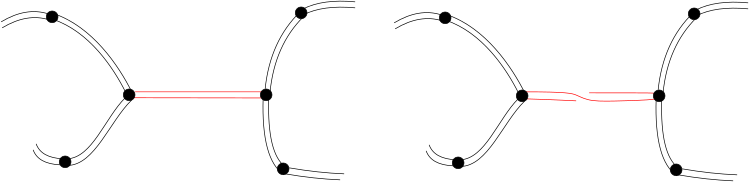
\includegraphics[scale=0.4]{twist}
		\centering
		\caption{The red edge is twisted in two different ways}
	\end{figure}
	
	
	We describe algorithm of choosing the twists, which constitutes the desired bijection.
	
	We start by exploring how twist affects the type of the root in different settings.
	
	\begin{itemize}
		\item[\textbf{Case 1}] \emph{The root connects corners from two disconnected components}.
		
		The root twist results in the isomorphic map. In any case the added root is a \textbf{bridge}. Also note (we'll need this fact later), that connecting two unicellular components gives a unicellular component too.

		\item[\textbf{Case 2}] \emph{The root connects corners from the same face.}
		
		 First, we depict the traversed face before adding the root:
		
		\begin{figure}[H]
			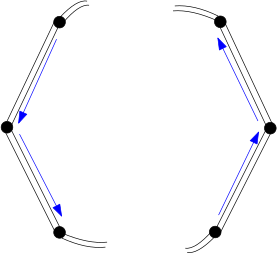
\includegraphics[scale=0.4]{traversed_face}
			\centering
			\caption{A traversed face}
		\end{figure}
		
		Then depending on the twist, we either add one more face (in that case the added root is a \textbf{border}) or we keep the number of faces unchanged (the added root is a \textbf{twist}):
		
		\begin{figure}[H]
			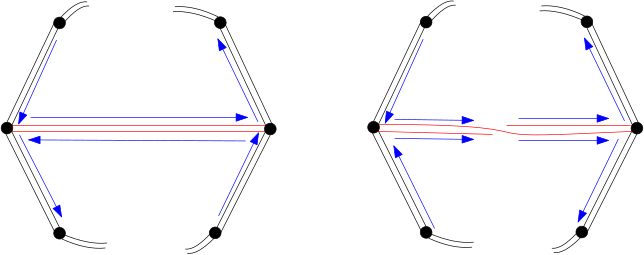
\includegraphics[scale=0.4]{connecting_corners_of_one_face}
			\centering
			\caption{Connecting corners of one face. The added bridge on the left and the added twist on the right.}
		\end{figure}
		
		Note, that the border doesn't change the orientability of the map, while adding a twist always gives a non-orientable map.
		
		\item[\textbf{Case 3}] \emph{The root connects corners from different faces but from the same connected component}.
		
		We diagrammatically depict the traversed faces, containing the added root:
		
		\begin{figure}[H]
			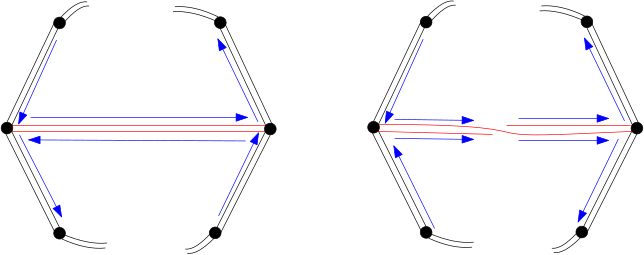
\includegraphics[scale=0.4]{connecting_corners_of_one_face}
			\centering
			\caption{Connecting different faces.}			
		\end{figure}
		
		In both cases we decrease the number of faces by one and the added root is a \textbf{handle}. But the twist changes the traversing direction of one of the faces. So if the map without the added root is oriented, only one of the resulting maps is oriented.
	\end{itemize}

	First, we show how to make an oriented rooted map from unicellular unhandled one. We start the root adding process from $v$ trivial components and by induction we assume, that on each step all the connected components are orientable.
	\begin{itemize}
		\item If we encounter \textbf{Case 1} during the root addition process, we choose any of the twists.
		
		\item If we encounter \textbf{Case 2}, we twist the ribbon in a way to get a border.
		
		\item If we encounter \textbf{Case 3}, we twist the ribbon in unique available way to keep the corresponding component orientable. 
	\end{itemize}

	Now we give an algorithm of getting an unicellular unhandled map from an oriented rooted map. Again, we do the root addition process. Our strategy is to avoid the \textbf{Case 3}, since it always results in adding a handle. Inductively we maintain the following property: every connected component is unicellular.
	
	\begin{itemize}
		\item If we encounter \textbf{Case 1}, we choose any of the twists. Note, that connecting to unicellular components results in an unicellular component too.
		
		\item If we encounter \textbf{Case 2}, we twist the ribbon i a way that gives a twisted root, thus keeping the number of faces of the component equal to $1$.
		
		\item We can not encounter \textbf{Case 3}, since it implies, that there is a component with at least $2$ faces, contradicting our induction hypothesis.
	\end{itemize}

	Careful analysis of both algorithms shows, that these transformations are inverse to each other.
\end{proof}

\begin{lemma}\label{lemma:moments_as_polynomial_in_c}
\begin{equation}
    \lim\limits_{m \to \infty}\langle \overline{L}_m, x^{2k} \rangle = c^{k + 1}\sum\limits_{\substack{\text{$M$ -- rooted, } \\ \text{oriented}, e(M) = k}}c^{-v(M)}
\end{equation}
\end{lemma}
\begin{proof}
    Similarly to the proof of \textbf{Proposition \ref{prop:variance}}, we use \cite{lacroix} \textbf{Corollary 4.17} to reformulate \textbf{Proposition \ref{prop:moments_and_h}} in terms of maps:
    \begin{multline}        
        \langle \overline{L}_{N}^{(\sfrac{2}{\alpha})}, x^{2k} \rangle = \frac{1}{N^{k + 1}}\sum\limits_{\mu \vdash 2k}h_{\mu, (2^k)}^{(2k)}(\alpha - 1)N^{l(\mu)} = \\
        = \frac{1}{N^{k + 1}}\sum\limits_{\substack{F(M) = (2k)}}(\alpha - 1)^{\eta(M)}N^{v(M)} = \sum\limits_{\substack{F(M) = (2k)}}(\alpha - 1)^{\eta(M)}N^{-2g(M)}
    \end{multline}
    And hence:
    $$ 
        \langle \overline{L}_m, x^{2k} \rangle = \sum\limits_{F(M) = (2k)}\left(\frac{2}{\beta_m} - 1\right)^{\eta(M)}N_m^{-2g(M)}.
    $$
    From \textbf{Lemma \ref{lemma:eta_bound}} it follows, that:
    $$
    \begin{cases}
        \lim\limits_{m \to \infty}\left(\frac{2}{\beta_m} - 1\right)^{\eta(M)}N_m^{-2g(M)} = c^{-2g(M)} & \text{ if $M$ is unhandled} \\
        \lim\limits_{m \to \infty}\left(\frac{2}{\beta_m} - 1\right)^{\eta(M)}N_m^{-2g(M)} = 0 & \text{ otherwise }
    \end{cases}
    $$
    Using \textbf{Lemma \ref{lemma:unhandled_to_oriented_bijection}}:
    \begin{multline*}
        \lim\limits_{m \to \infty}\langle \overline{L}_m, x^{2k} \rangle = \sum\limits_{ \substack{ M  \text{ -- unhandled}, \\ \text{unicellular}, e(M) = k}}c^{-2g(M)} = \\ = \sum\limits_{\substack{\text{$M$ -- rooted, } \\ \text{unicellular,} \\ \text{unhandled,} e(M) = k}}c^{-k + v(M) - 1} = c^{-k - 1}\sum\limits_{\substack{\text{$M$ -- rooted, } \\ \text{oriented}, e(M) = k}}c^{v(M)}.
    \end{multline*}
\end{proof}



\begin{proof}[Proof of \textbf{Proposition \ref{prop:moments}}]
    We show, that a quantity obtained in the \textbf{Lemma \ref{lemma:moments_as_polynomial_in_c}} satisfies a recurrence given in the statement of the proposition. All maps in this proof are oriented.
    
    Denote the set of oriented maps with $k$ edges by $\mathrm{M}(k)$. To derive a recurrence relation, we do one step of the root deletion process for a map $M \in \mathrm{M}(k)$.
    
    \begin{itemize}
    	\item[\textbf{Case 1}] \emph{$M$ splits into two connected components $M_1$ and $M_2$. We denote the set of such maps by $\mathrm{M}_{1}(k)$.}
    	
    	Conversely, we can obtain a unique map $\tilde{M}$ from two smaller maps $\tilde{M}_1$ and $\tilde{M_2}$ in a way reverse to the root deletion process.
    	
    	We connect the root corners of the map $\tilde{M}_1$ and $\tilde{M}_2$ by an edge. It splits the root corner of $\tilde{M}_1$ into two. Only one of them can be chosen as a root such that the deletion of the new root edge will give $M_1$ and $M_2$ back.
    	
    	\item[\textbf{Case 2}] \emph{The deletion of the root results in a connected map $M_1$. We denote the set of such maps by $\mathrm{M}_2(k)$}
    	
    	Conversely, we can obtain $2k - 1$ maps $\tilde{M}, \, \mathop{e}(M) = k$ from a map $\tilde{M}_1$ in a way reverse to the root deletion process.
    	
    	Note, that $\tilde{M}_1$ contains $2k - 3$ corners other than a root corner. We start by drawing a half-edge from a root corner, which splits it into two new ones. So we can connect the other half-edge to one of the $(2k - 3) + 2 = 2k - 1$. Again, the choice of the new root is uniquely determined. 
    \end{itemize}

	
    
	So for $k \geq 1$ we get a bijection:
    
    \begin{multline}\label{eq:oriented_maps_decomposition}
        \mathrm{M}(k) = \mathrm{M}_1(k) \sqcup \mathrm{M}_2(k) \longleftrightarrow \\ 
        \longleftrightarrow\left(\bigsqcup_{r + s = k - 1}\mathrm{M}(r)\times \mathrm{M}(s)\right) \sqcup \left(\{1,\,  \ldots,\, 2k - 1\} \times \mathrm{M}(k - 1)\right).
    \end{multline}

    Now denote:
    $$
        a_k = c^{k + 1}\sum\limits_{M \in \mathrm{M}(k)}c^{-v(M)}.
    $$
    
    Clearly, $a_0 = 1$, and, using (\ref{eq:oriented_maps_decomposition}), for $k \geq 1$ we get
    \begin{multline}
		a_k = \sum\limits_{M \in \mathrm{M_1}(k)}c^{k + 1 - \mathop{v}(M)} + \sum\limits_{N \in \mathrm{M_2}(k)}c^{k + 1 - \mathop{v}(N)} = \\
		 = \sum\limits_{\substack{r + s = k - 1 \\ M_1 \in \mathrm{M}(r) \\ M_2 \in \mathrm{M}(s)}}c^{r + 1 + \mathop{v}(M_1)}c^{s + 1 \mathop{v}(M_2)} + \sum\limits_{N_1 \in \mathrm{M}(k - 1)}(2k - 1)c\cdot c^{(k - 1) + 1 + \mathop{v}(N_1)} = \\
		 = \sum\limits_{r + s = k - 1}a_ra_s + c(2k - 1)a_{k - 1},
    \end{multline}
    which coincides with the reccurence for $M_{2k}$.
\end{proof}

\begin{proof}
	It's a corollary of \textbf{Proposition \ref{prop:moments_and_h}} (shows, that all moments of $\overline{L}_m$ exist), \textbf{Proposition \ref{prop:moments}} and \textbf{Theorem 3.5} from \cite{randmatrgeneral}.
\end{proof}

\begin{proof}[Proof of the \textbf{Theorem \ref{theorem:main}}]
	The brief plan of the proofs is the following:
	\begin{itemize}
		\item Show, that numbers $M_k$ satisfy the Carleman's condition.
		
		\item It follows from \textbf{Theorem 3.5} of \cite{randmatrgeneral}, that there exits a unique measure $L$, such that $\langle L, x^k \rangle = M_k$ and $\overline{L}_m$ weakly converges $L$.
		
		\item Show, that $\langle L_m, x^k \rangle$ converges in probability to $M_k = \langle L, x^k \rangle$.
		
		\item Theorem statement follows from \textbf{Theorem 3.7}, part \emph{ii)} of \cite{randmatrgeneral}.
	\end{itemize}
	For brevity, denote $a_k \coloneqq M_{2k}$. Note, that for $k \geq 1$:
	\begin{multline}
		a_{k} = \left(\sum\limits_{\substack{r + s = k - 1 \\ r, s \geq 1}}a_ra_s\right) + 2a_0a_k + c(2k - 1)a_{k - 1} = \left(\sum\limits_{\substack{r + s = k - 1 \\ r, s \geq 1}}a_ra_s\right) + (c(2k - 1) + 2)a_{k - 1} \leq \\ \leq (c + (2k - 1) + 2) \sum\limits_{r + s = k - 1}a_ra_s
	\end{multline}\todo{$a_k$ turned into $a_{k-1}$}
	Denote $C = c + (2k - 1) + 2$. Define a sequence:
	$$
	\begin{cases}
		b_k =  C \sum\limits_{r + s = k - 1}b_rb_s  & k \geq 1 \\
		b_k = 1 & k = 0
	\end{cases}
	$$
	Clearly, $a_k \leq b_k$ and a sequence $\frac{b_k}{C^k}$ satisfies Catalan's numbers recurrence, so using the Stirling's approximation:
	
	$$
	a_k = C^k\frac{1}{k + 1}\binom{2k}{k}C^k \sim \frac{C^k2^{2k}}{\sqrt{2\pi k}} \coloneq c_k,
	$$
	Clearly:
	$$
		\sum\limits_{k = 1}^{\infty}c_k^{-\sfrac{1}{2k}} = +\infty,
	$$
	so $M_k$ satisfies Carleman's condition. \todo{but $C$ depends
        on $k$. ooops...}
	
	To show, that $\langle L, x^k\rangle$ converges in probability to $M_k$ we note that:
	
	\begin{multline*}
		\prob{|\langle L_m, x^k \rangle - M_k| > \epsilon} \leq  \\ \leq	\prob{\left|\langle L_m, x^k \rangle - \langle\overline{L}_m, x^k\rangle\right| > \frac{\epsilon}{2}} + \prob{\left|\langle\overline{L}_m, x^k\rangle - M_k\right| > \frac{\epsilon}{2}}.
	\end{multline*}
	The latter summand is eventually $0$ by \textbf{Proposition \ref{prop:moments}}. To estimate the first summand we use the Tchebysheff inequality and \textbf{Proposition \ref{prop:variance}}:
	$$
		\prob{\left|\langle L_m, x^k \rangle - \langle\overline{L}_m, x^k\rangle\right|} \leq \frac{\Var{\langle L_m, x^k \rangle}}{(\sfrac{\epsilon}{2})^2} \longrightarrow 0.
	$$
\end{proof}


\bibliographystyle{alpha}
\bibliography{refs.bib}

\end{document}

